\subsection{Lab Book Excerpts}

\textit{Note: This section requires one-page excerpts from handwritten lab book for each of the following eight headings. Each excerpt should be scanned at high resolution (minimum 300 DPI) and inserted as a full-page figure. Lab book excerpts must be legible, dated, and demonstrate the engineering process followed during subsystem development.}

\stepcounter{subsubsection}  % Increment the section number manually
\subsubsection*{\thesubsubsection\hspace{1em} Design Constraints}

% Insert scanned lab book excerpt showing analysis of design constraints including:
% - Component availability limitations (electret microphone selection)
% - Single-supply voltage constraint (0-5V operation)
% - Frequency selectivity vs. component tolerance analysis
% - Processing resource constraints (ESP32 GPIO limitations)
% - Acoustic environment characterization

\begin{figure}[H]
\centering
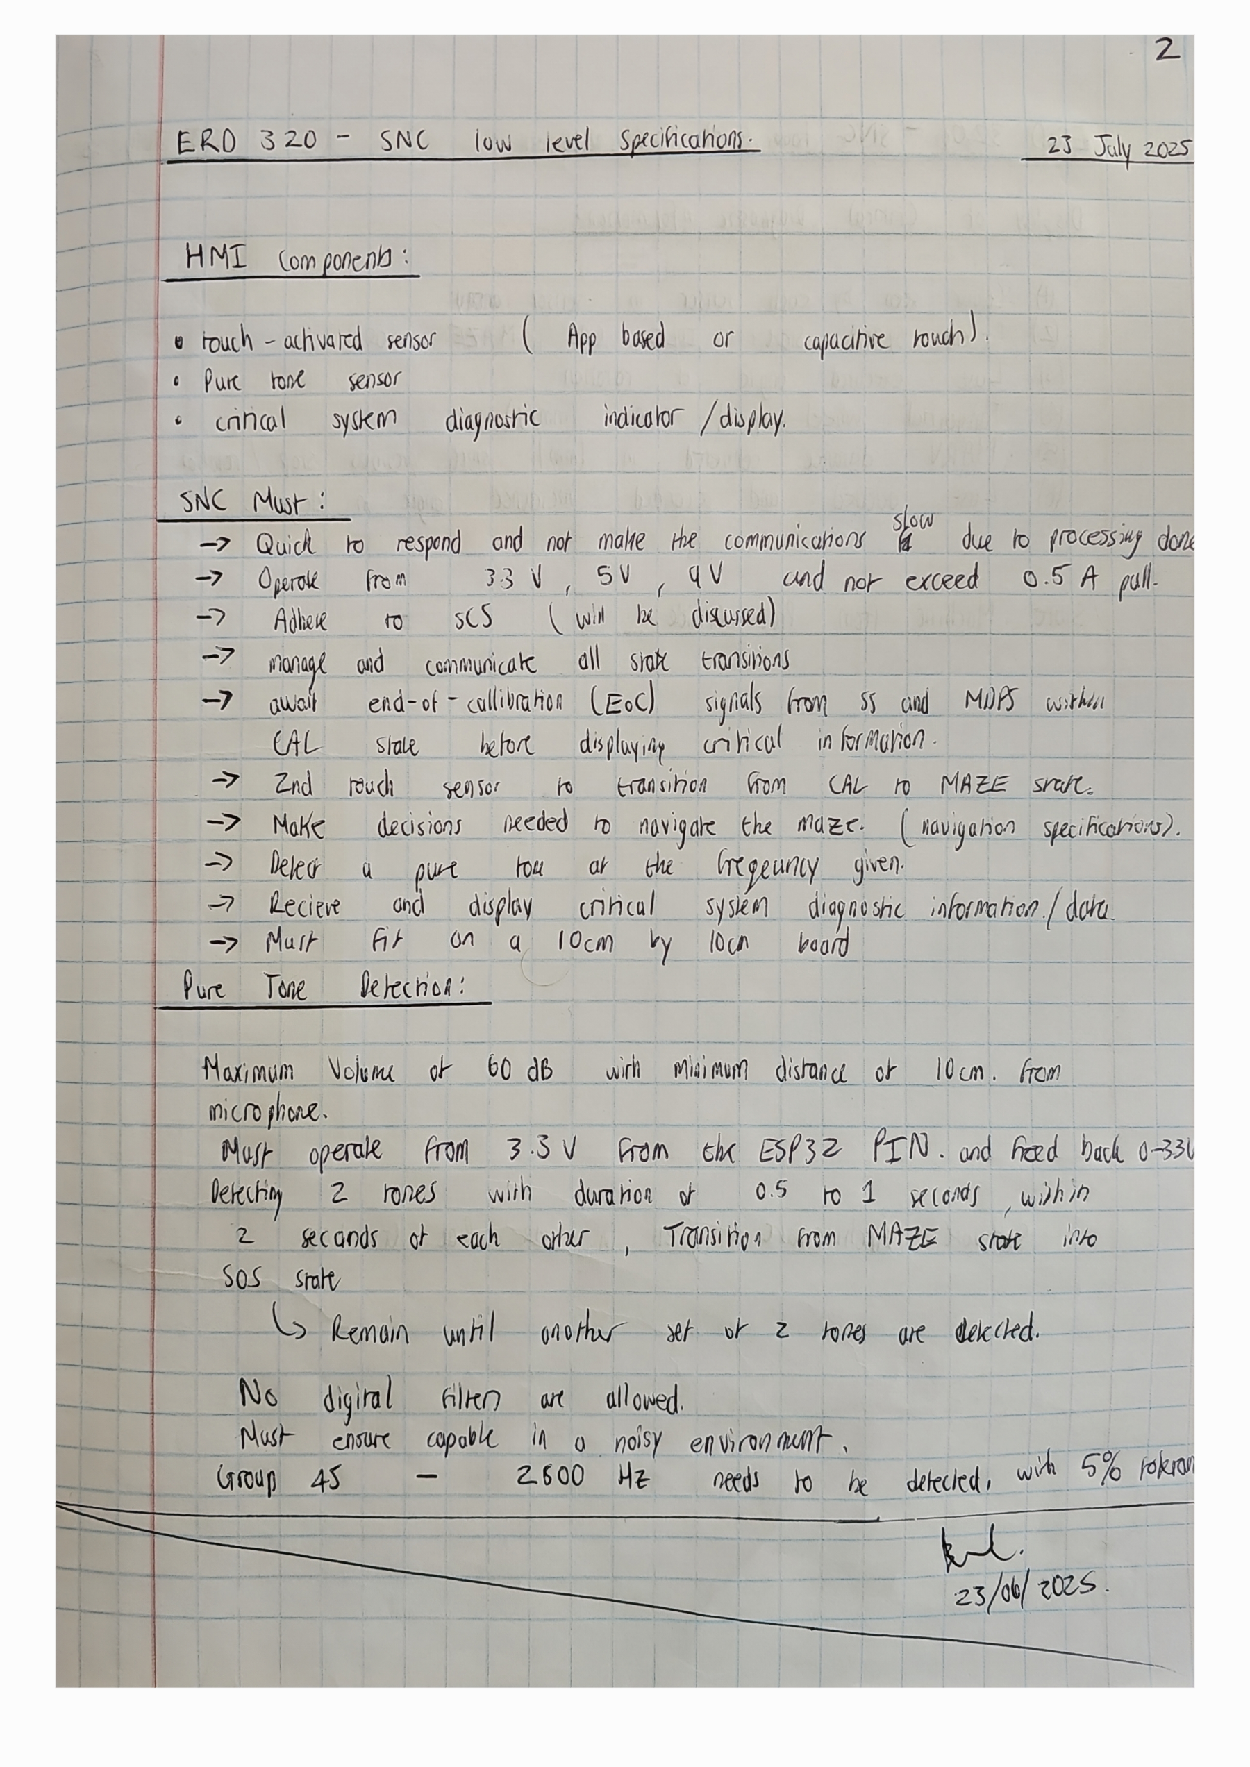
\includegraphics[width=0.9\textwidth]{01_SNC/Labbook/labbook_constraints.pdf}
\caption{Lab book excerpt: Design Constraints analysis for SNC subsystem}
\label{fig:labbook-constraints}
\end{figure}

\stepcounter{subsubsection}  % Increment the section number manually
\subsubsection*{\thesubsubsection\hspace{1em} Trade-offs}

% Insert scanned lab book excerpt documenting trade-off analyses including:
% - Filter order vs. circuit complexity (2nd vs. 4th order decision)
% - Microphone sensitivity vs. noise floor trade-off
% - Envelope time constant vs. responsiveness
% - Comparator threshold setting analysis

\begin{figure}[H]
\centering
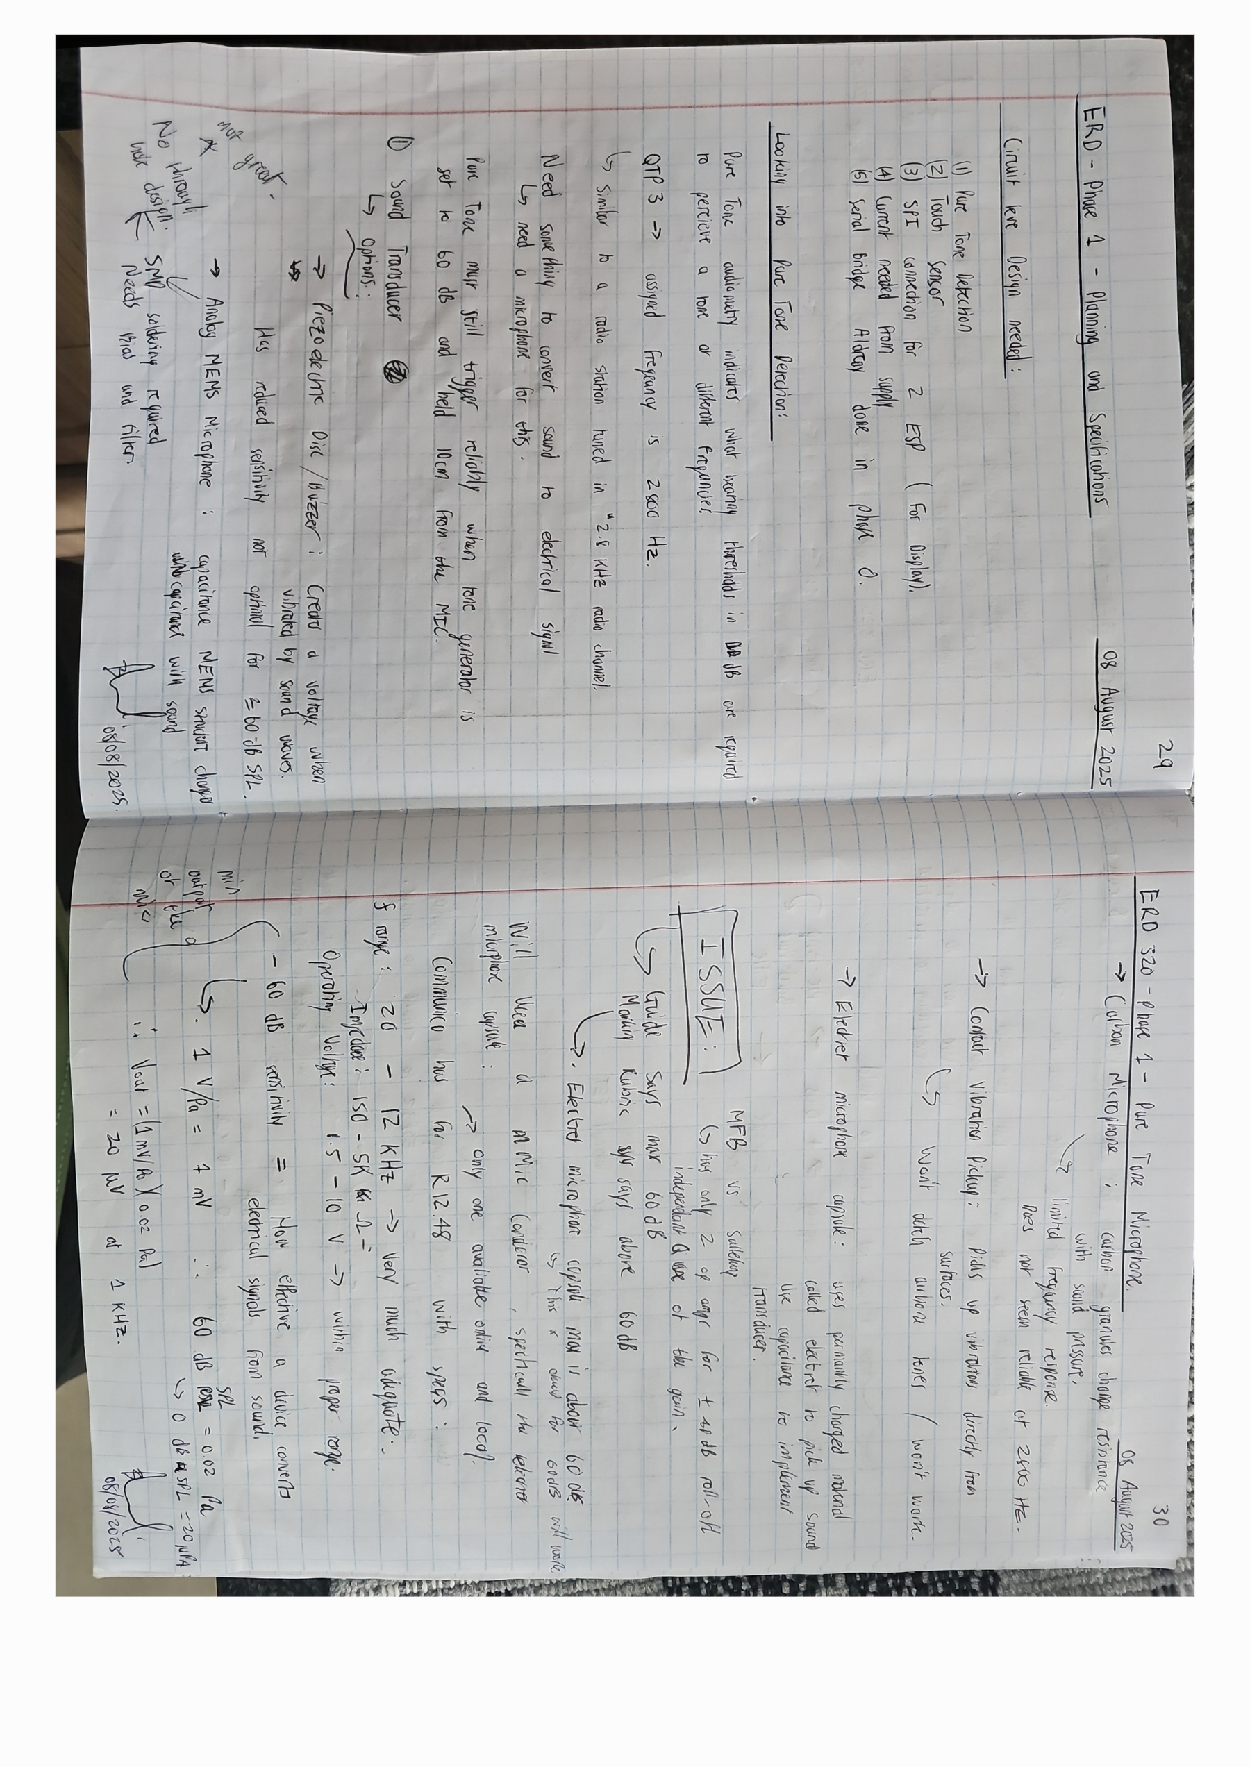
\includegraphics[width=0.9\textwidth]{01_SNC/Labbook/labbook_tradeoffs.pdf}
\caption{Lab book excerpt: Trade-offs analysis for pure tone detection circuit}
\label{fig:labbook-tradeoffs}
\end{figure}

\stepcounter{subsubsection}  % Increment the section number manually
\subsubsection*{\thesubsubsection\hspace{1em} Engineering tools}

% Insert scanned lab book excerpt listing engineering tools used:
% - LTspice XVII for analogue circuit simulation
% - Arduino IDE / PlatformIO for ESP32 firmware development
% - Logic analyzer for protocol timing verification
% - Oscilloscope for analogue signal chain measurement
% - Function generator for tone testing
% - Browser DevTools for web dashboard development

\begin{figure}[H]
\centering
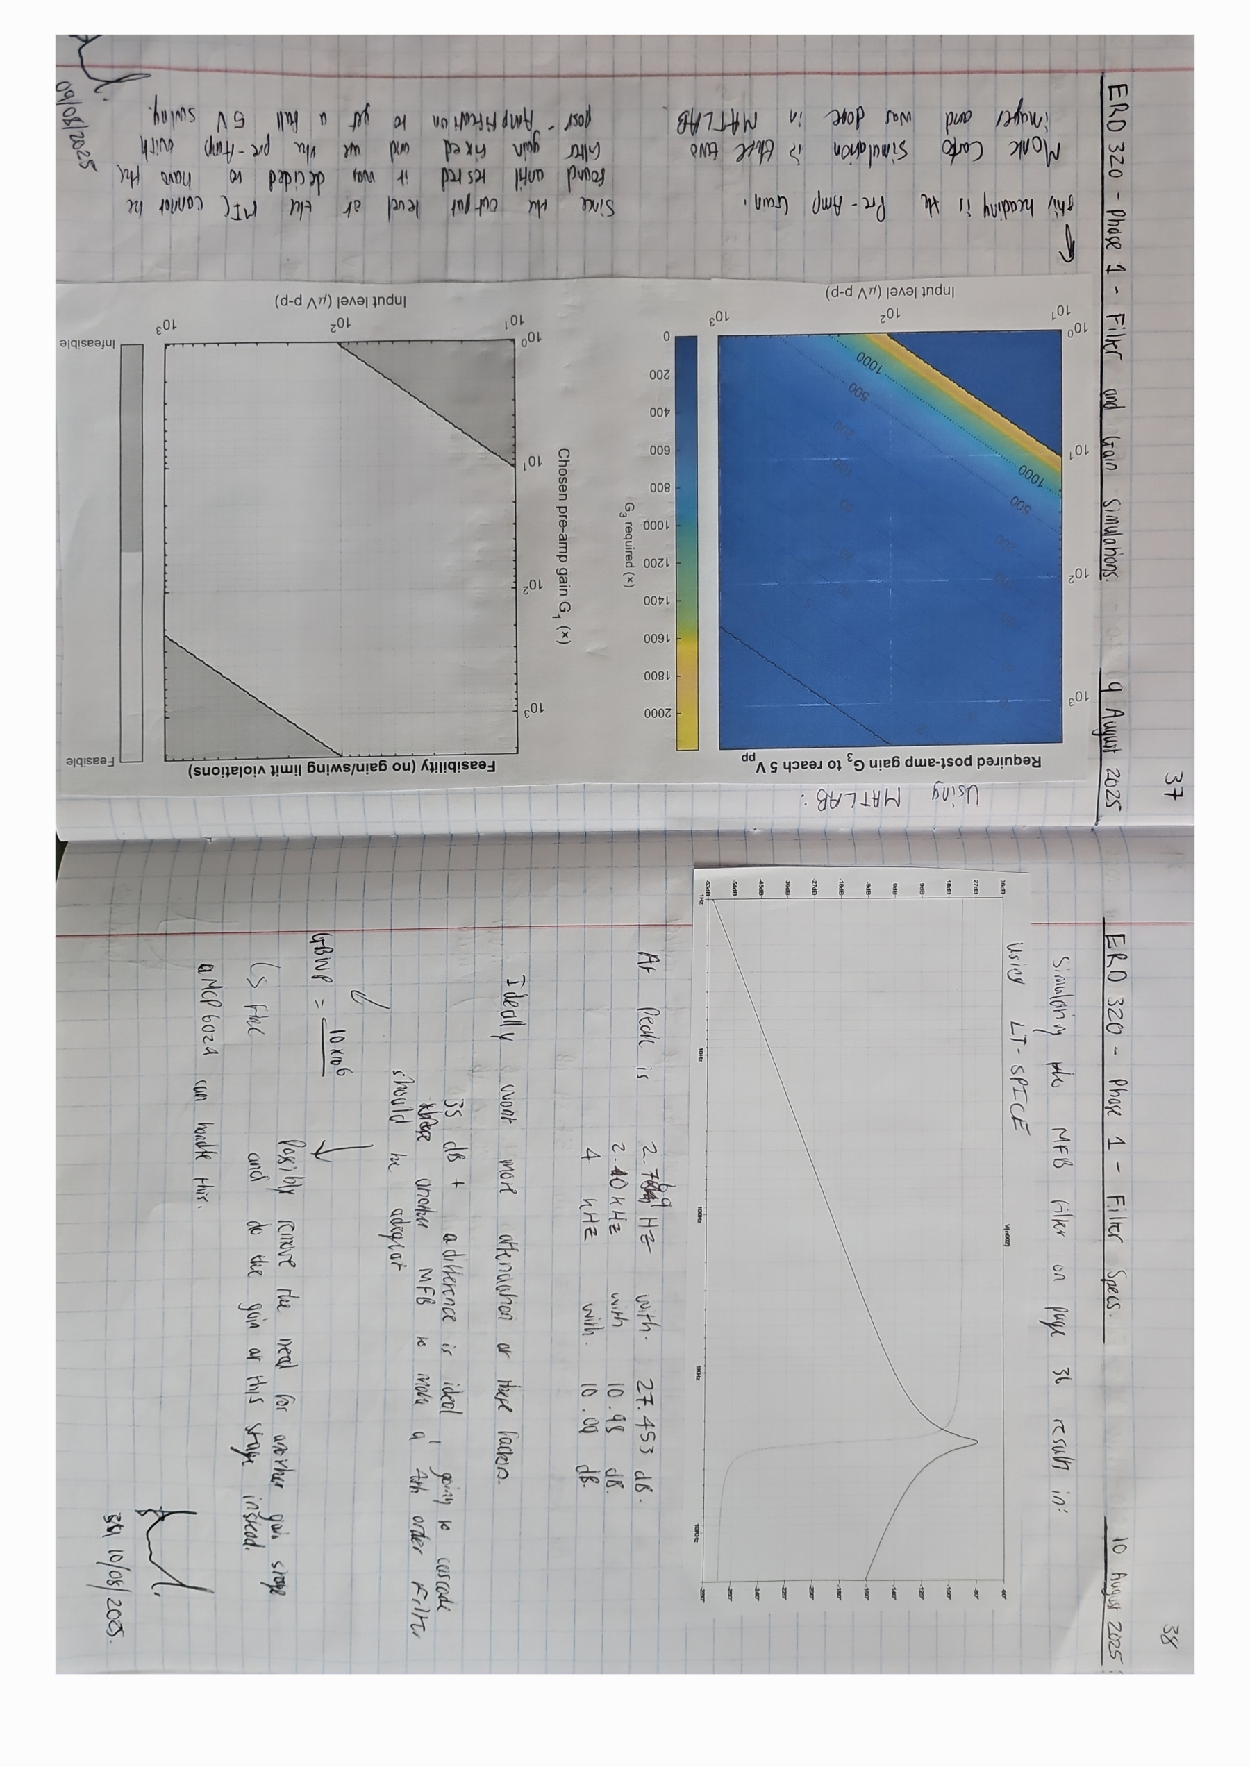
\includegraphics[width=0.9\textwidth]{01_SNC/Labbook/labbook_tools.pdf}
\caption{Lab book excerpt: Engineering tools and test equipment used}
\label{fig:labbook-tools}
\end{figure}

\stepcounter{subsubsection}  % Increment the section number manually
\subsubsection*{\thesubsubsection\hspace{1em} Engineering methods}

% Insert scanned lab book excerpt describing engineering methods:
% - Phase 0 waterfall approach for pure tone detection validation
% - Phase 1-3 iterative/agile firmware development sprints
% - Parameter sweep methodology for filter optimisation
% - Test-driven integration approach (unit → interface → subsystem → full system)

\begin{figure}[H]
\centering
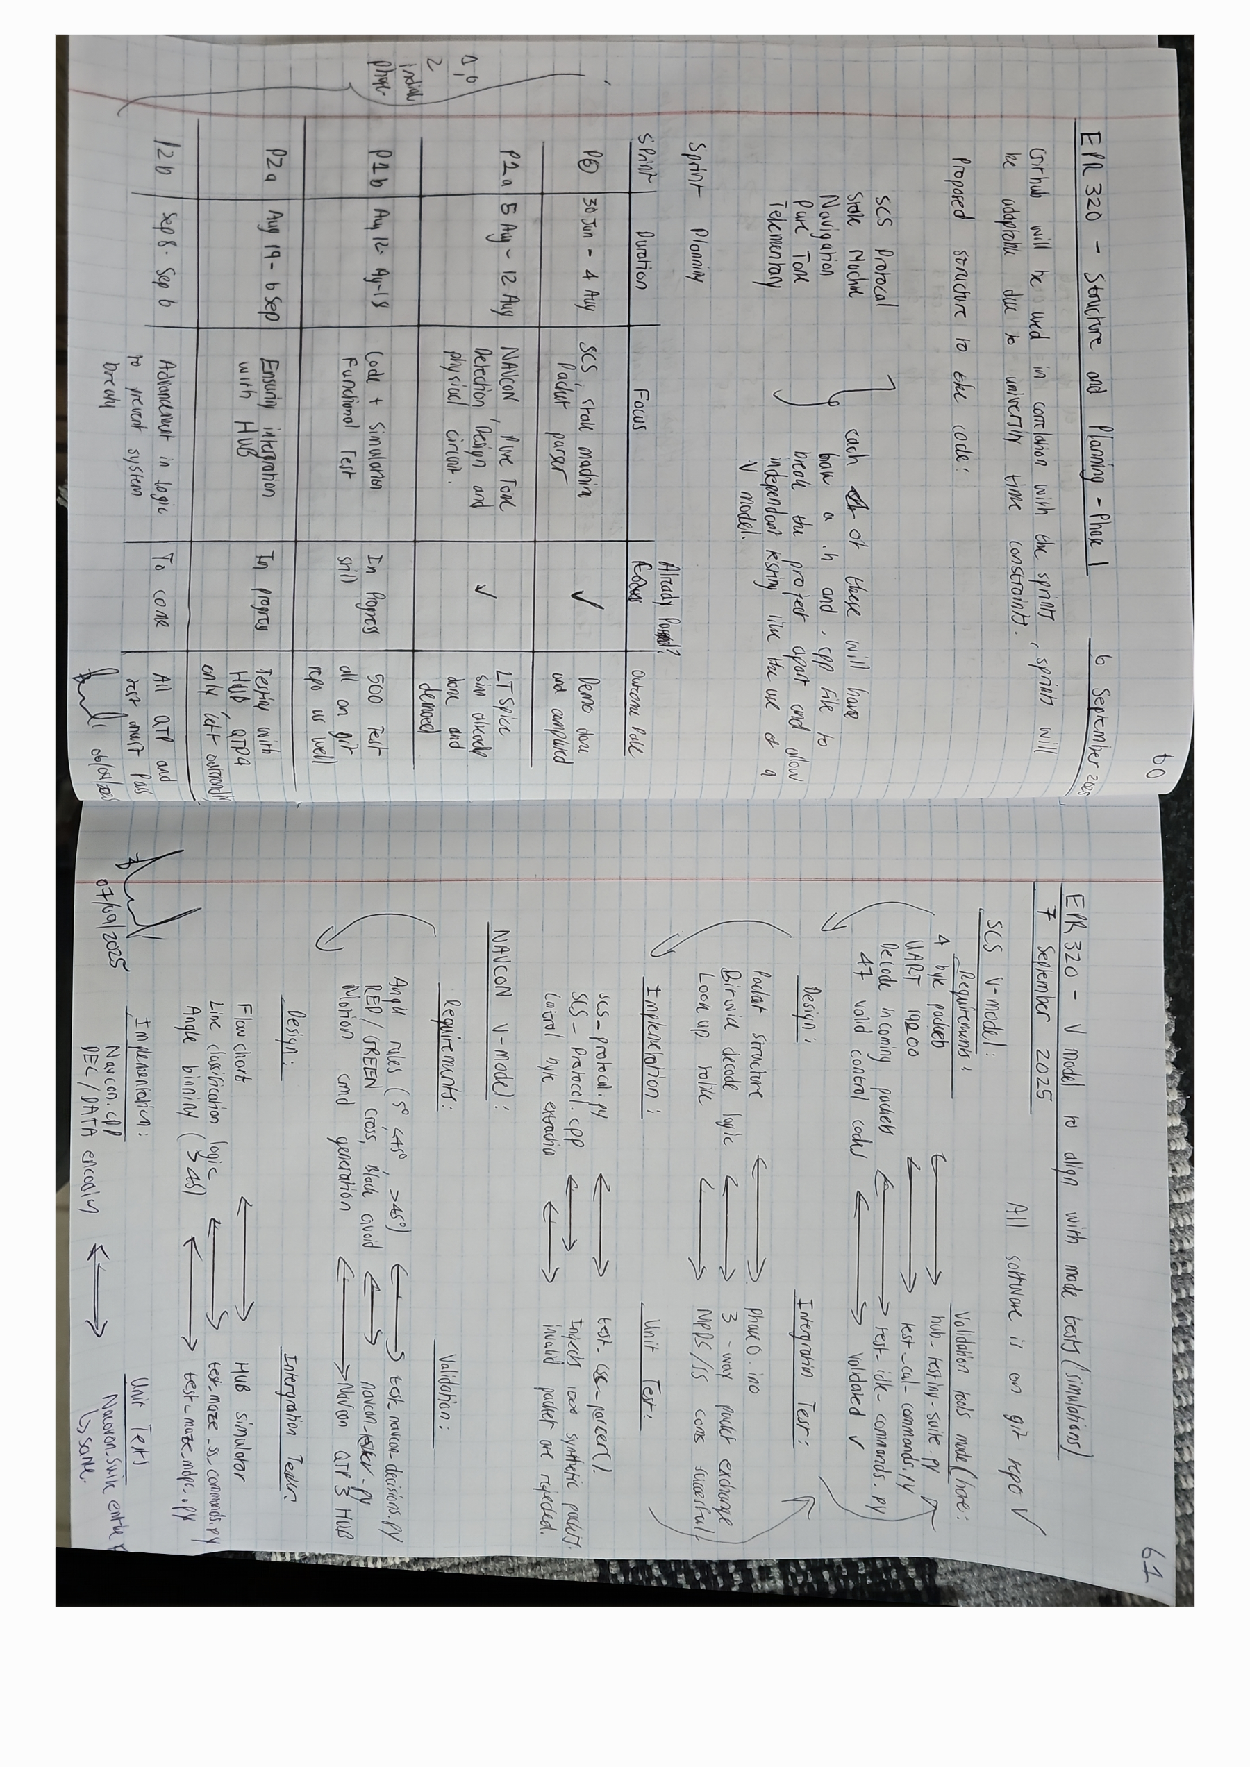
\includegraphics[width=0.9\textwidth]{01_SNC/Labbook/labbook_methods.pdf}
\caption{Lab book excerpt: Engineering methods and development process}
\label{fig:labbook-methods}
\end{figure}

\stepcounter{subsubsection}  % Increment the section number manually
\subsubsection*{\thesubsubsection\hspace{1em} Statements of requirements}

% Insert scanned lab book excerpt with requirements specification:
% - PTD-R-01 through PTD-R-07 (pure tone detection requirements)
% - State machine transition requirements
% - SCS protocol compliance requirements
% - NAVCON functional requirements
% - WiFi telemetry and HMI requirements

\begin{figure}[H]
\centering
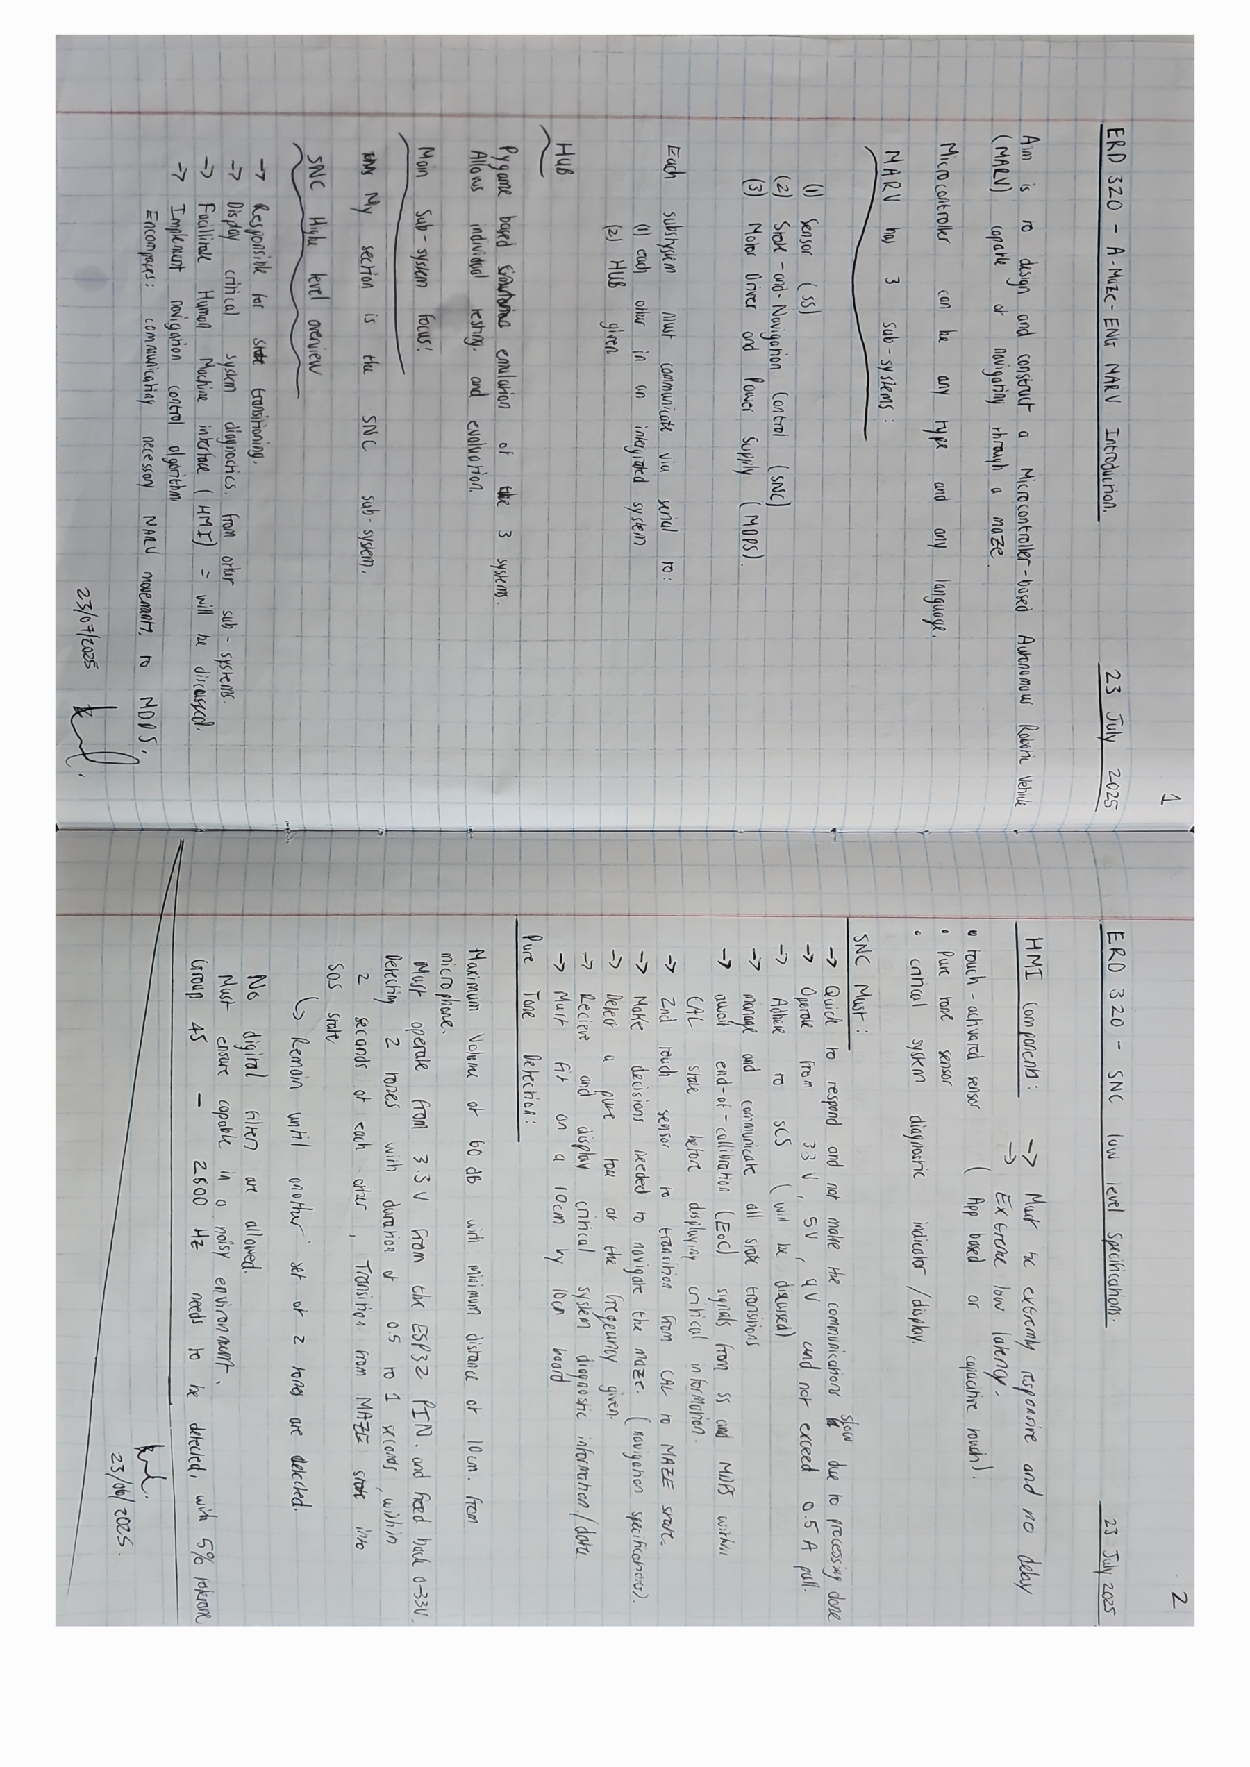
\includegraphics[width=0.9\textwidth]{01_SNC/Labbook/labbook_requirements.pdf}
\caption{Lab book excerpt: Requirements specification for SNC subsystem}
\label{fig:labbook-requirements}
\end{figure}

\stepcounter{subsubsection}  % Increment the section number manually
\subsubsection*{\thesubsubsection\hspace{1em} Development}

% Insert scanned lab book excerpt documenting development activities:
% - Circuit schematic sketches (microphone biasing, \gls{mfb} filter stages, envelope detector)
% - Component value calculations with design equations
% - Breadboard prototype photos/sketches
% - Initial testing observations and issues encountered
% - Iterative design refinements

\begin{figure}[H]
\centering
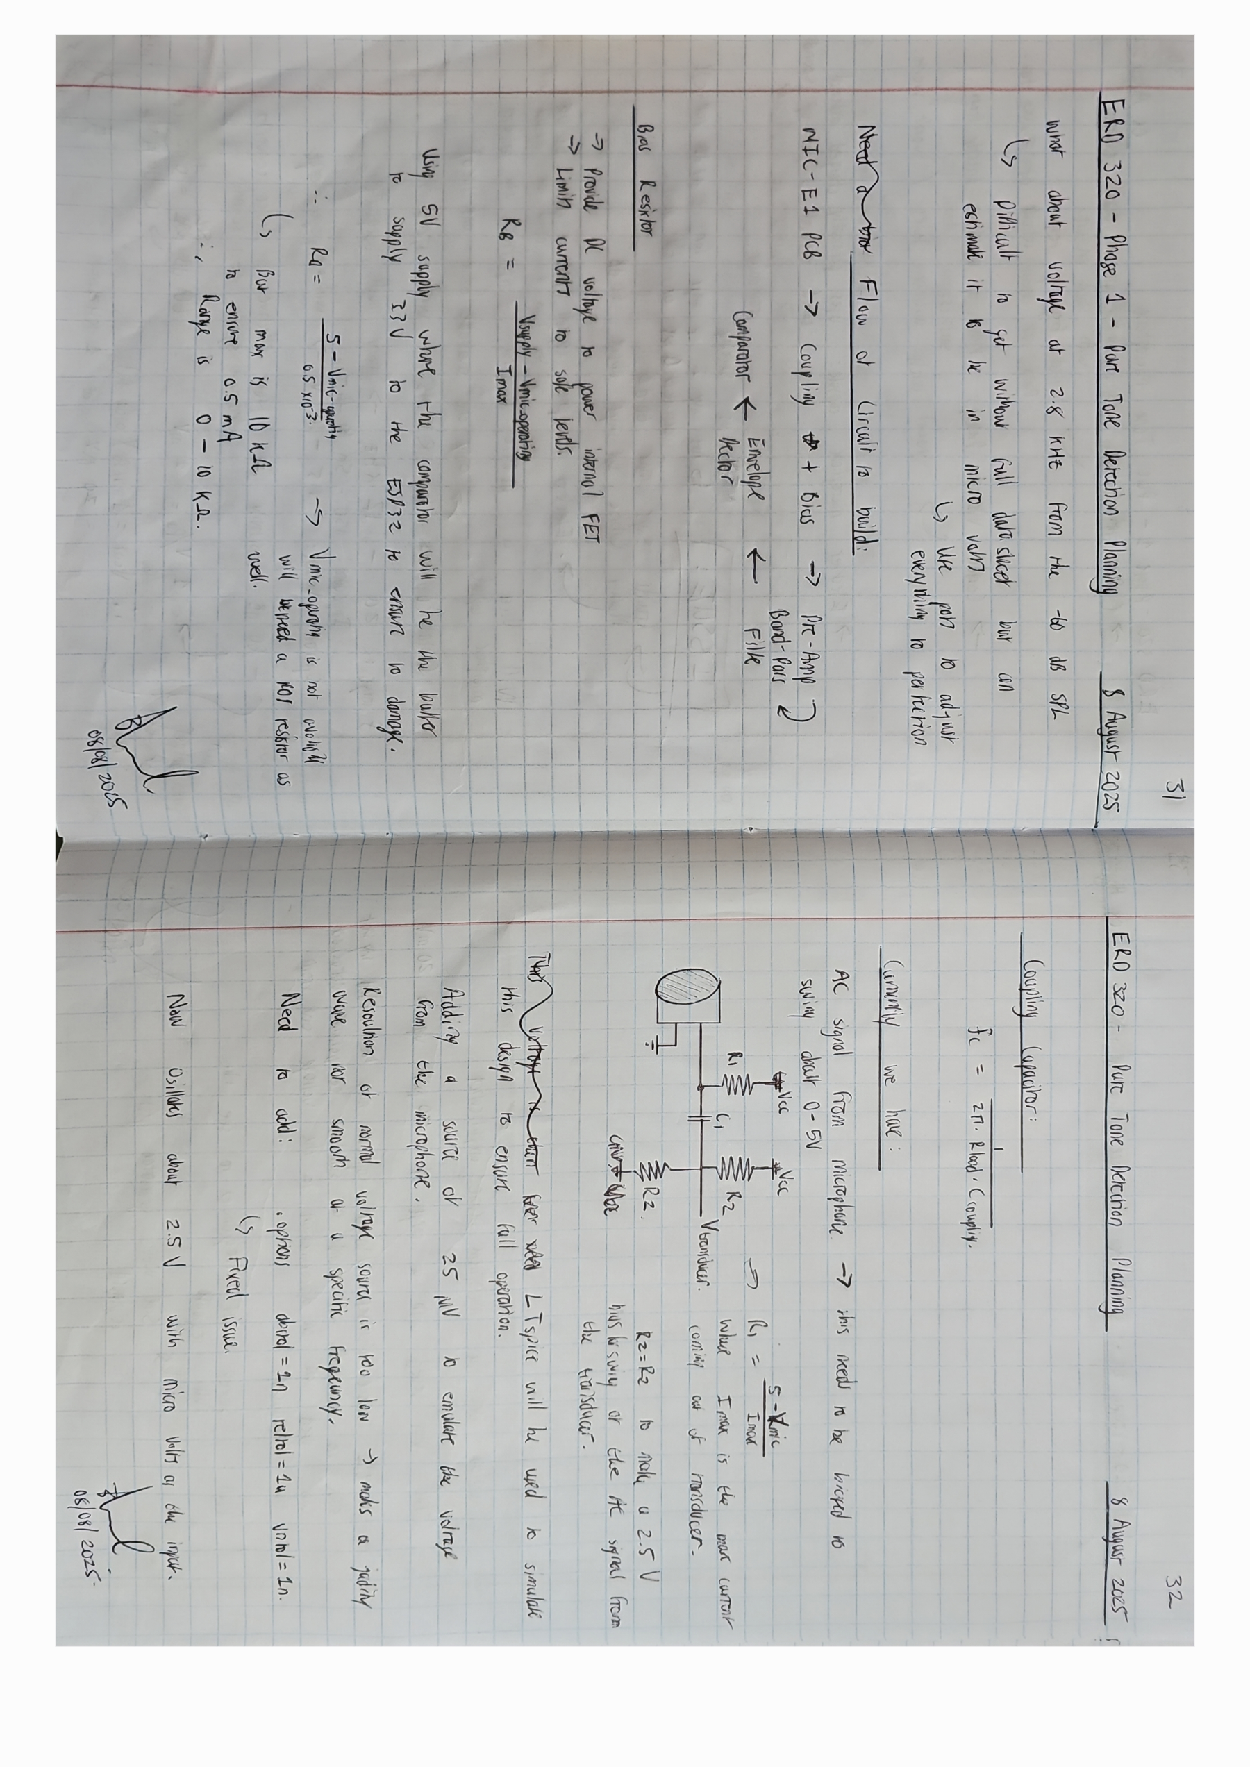
\includegraphics[width=0.9\textwidth]{01_SNC/Labbook/labbook_development.pdf}
\caption{Lab book excerpt: Development activities and circuit prototyping}
\label{fig:labbook-development}
\end{figure}

\stepcounter{subsubsection}  % Increment the section number manually
\subsubsection*{\thesubsubsection\hspace{1em} Simulations}

% Insert scanned lab book excerpt showing simulation results:
% - LTspice frequency response plots (Bode plots showing 2800 Hz passband)
% - Transient simulation of envelope detector with 2800 Hz input
% - Q-factor and bandwidth calculations from simulation data
% - Component tolerance sensitivity analysis results
% - Comparator threshold crossing timing

\begin{figure}[H]
\centering
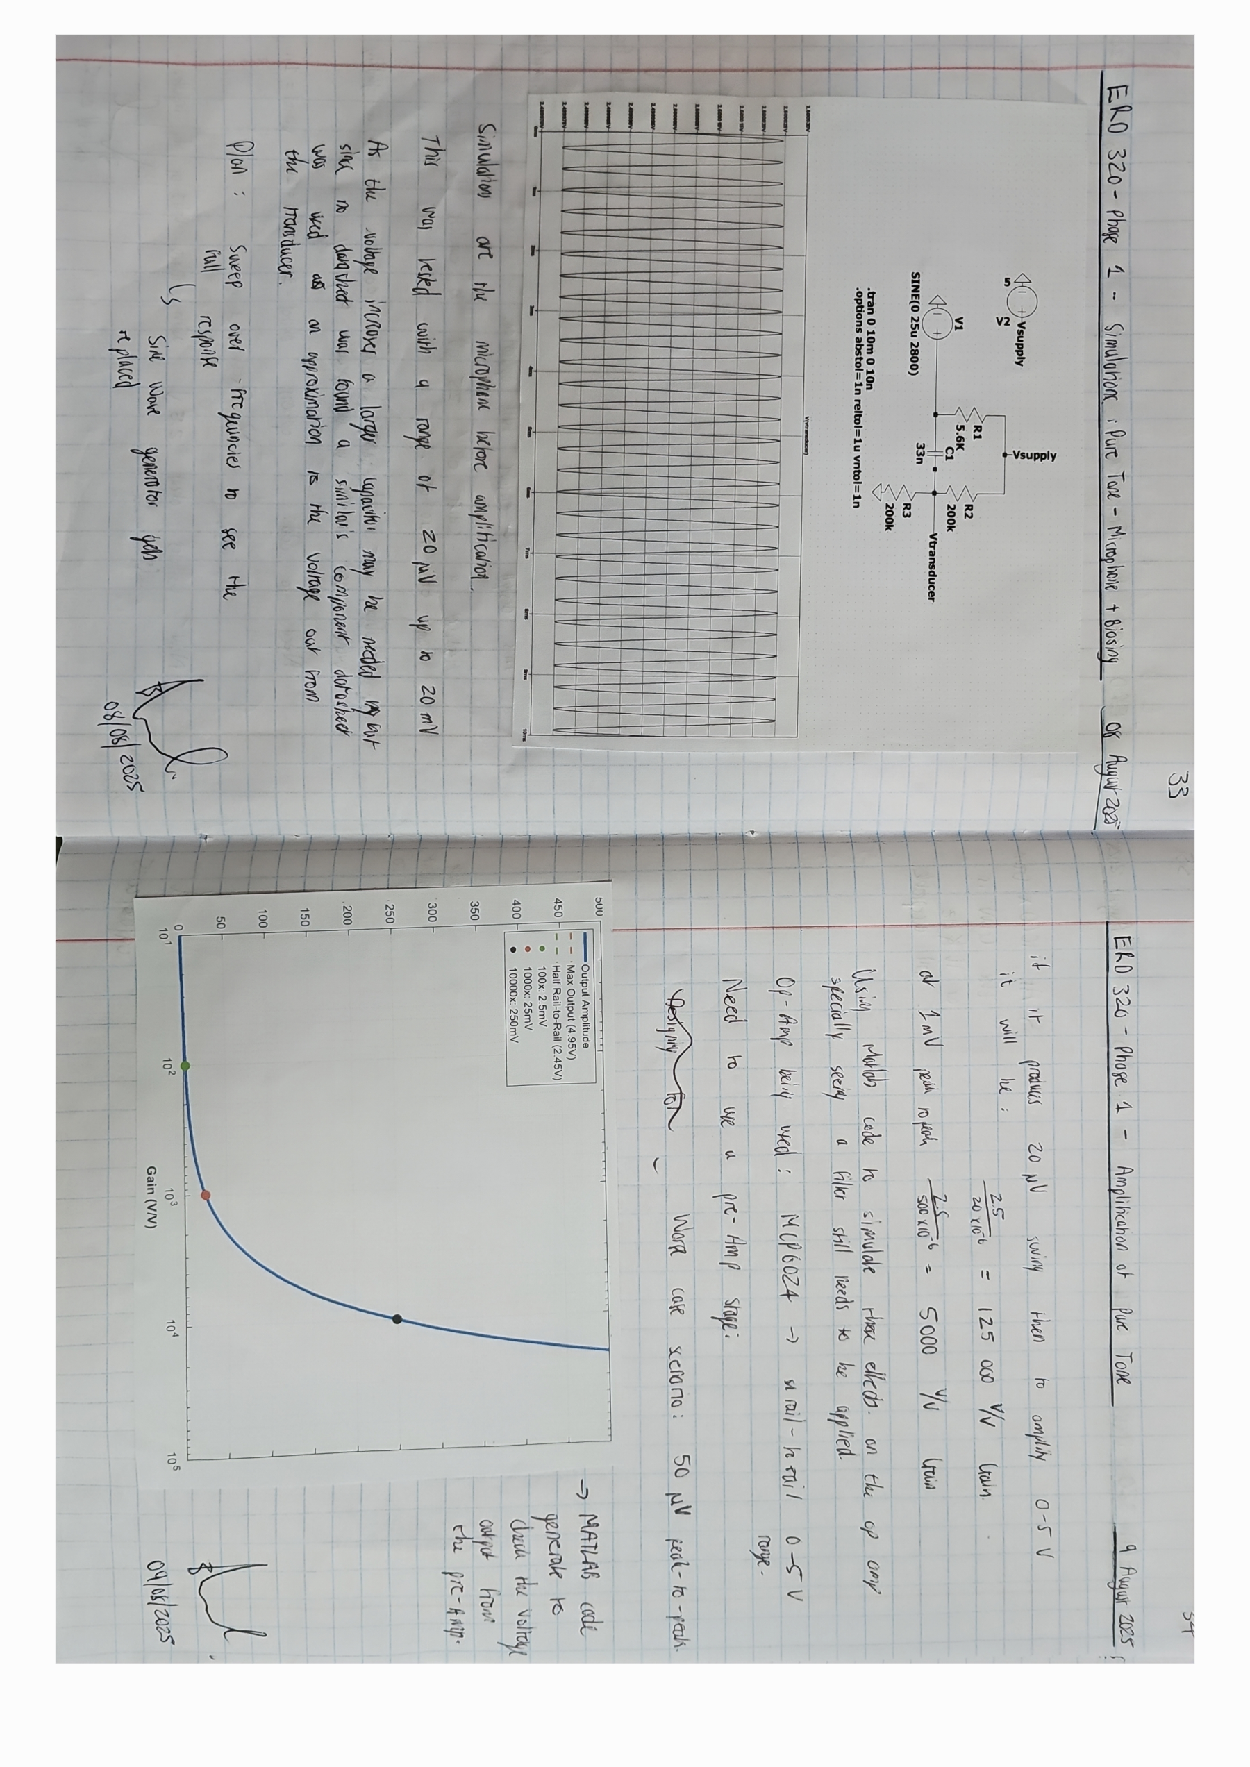
\includegraphics[width=0.9\textwidth]{01_SNC/Labbook/labbook_simulations.pdf}
\caption{Lab book excerpt: SPICE simulation results and analysis}
\label{fig:labbook-simulations}
\end{figure}

\stepcounter{subsubsection}  % Increment the section number manually
\subsubsection*{\thesubsubsection\hspace{1em} Approach to coding and testing}

% Insert scanned lab book excerpt describing firmware development approach:
% - State machine implementation strategy (IDLE/CAL/MAZE/SOS)
% - NAVCON decision logic structure and rule hierarchy
% - SCS protocol parser implementation notes
% - Unit testing approach for packet validation
% - Integration testing with HUB simulator
% - Debugging strategies and tools (serial monitor, logic analyzer traces)

\begin{figure}[H]
\centering
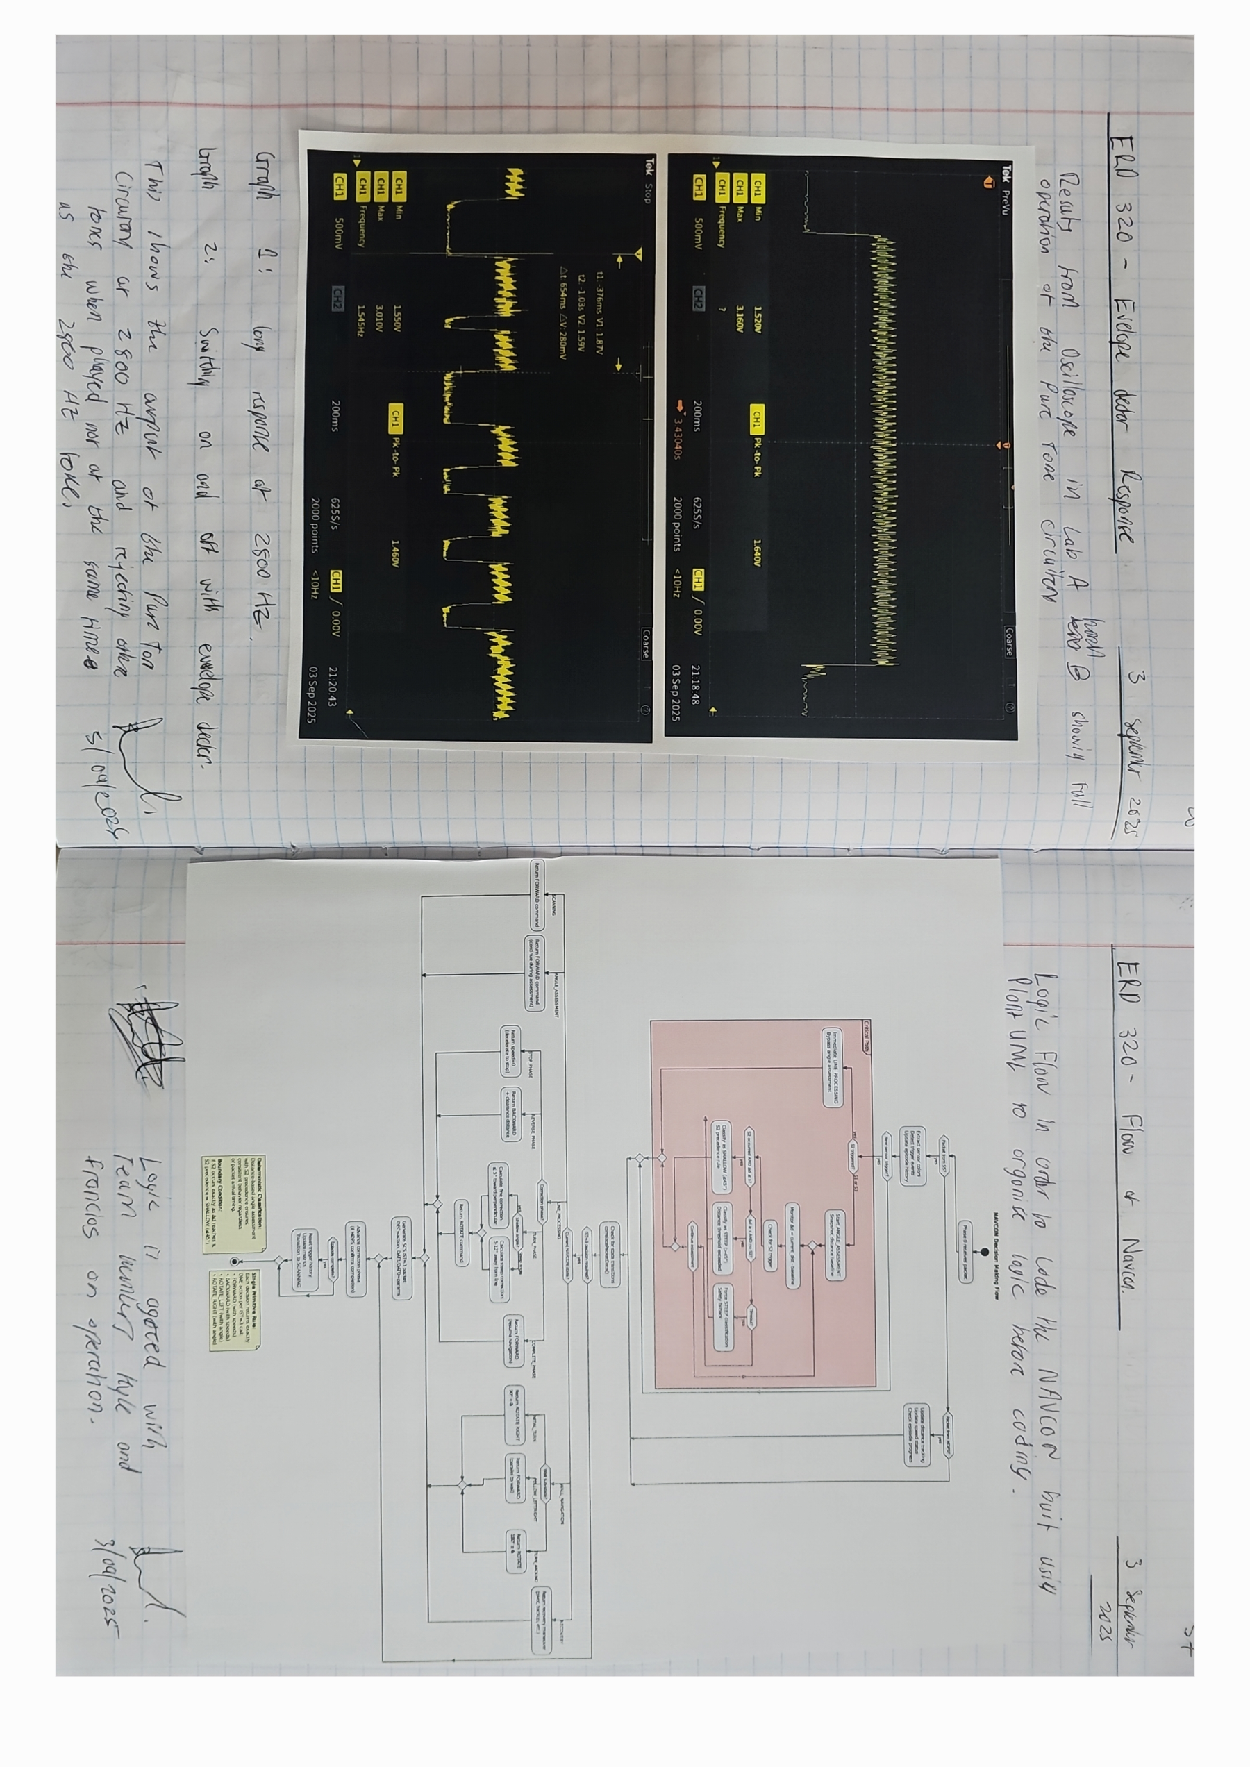
\includegraphics[width=0.9\textwidth]{01_SNC/Labbook/labbook_coding.pdf}
\caption{Lab book excerpt: Approach to firmware coding and testing}
\label{fig:labbook-coding-testing}
\end{figure}

